\section{Reinforcement learning algorithm}\label{sec:reinforcement_learning}

The agent based mode described in Section~\ref{sec:agent_based_model} describes
how the agents can interact with the environment.
The next step is to describe how the agents can learn from their interactions.
A reinforcement learning algorithm is described in this section where the agents
update their service rates based on the utilities they receive from the
queueing system.
The concepts described in Section~\ref{sec:queueing_section} and
Section~\ref{sec:agent_based_model} are incorporated in the reinforcement
learning algorithm so that the agents decide how fast they should serve the
customers in order to maximise their own utility.

The reinforcement learning algorithm is a policy iteration algorithm where
the agents update their service rates based on the utilities they receive
from the queueing system.
The service rates will be referred to as the policy in this section.
A policy is a set of service rates for every server for each possible state
they can be in.
The following pseudo-code describes the reinforcement learning algorithm.
At each time step, the agent receives a utility $U$ from the queueing system
and updates its service rate $s$ based on the utility it received.
Recall from Section~\ref{sec:agent_based_model} that each agent (server) has
a different service rate for each possible state they can be in.

\vspace*{0.5cm}

\begin{lstlisting}
Choose an initial policy
Run simulation with current policy
Calculate initial utility U_current
For each time step
    1. Choose a server k
    2. Choose a state (u, v)
    3. Update policy for server k and state (u, v)
    4. Rerun simulation
    5. Calculate utility U_new
    6. If utility U is higher than previous utility
        - Update service rate s
        - Update U_current to U_new

\end{lstlisting}

% TODO: Cite archive of pseudo-code and results

The total number of time steps is a parameter that needs to be set to a high
enough value to ensure that the agents have enough time to learn from their
interactions with the queueing system.
Additionally, in order to eliminate any stochasticity from the simulation
at each time step the simulation is run for a fixed runtime and a fixed number
of trials.
Furthermore, when choosing a new policy for a server and a state, the
algorithm will choose a new policy that is within a certain range of the
current policy and that cannot be below zero.

Consider an example of a queueing system with \(2\) servers and the following
set of states:

\begin{equation}
    \mathcal{S} = \{(0, 0), (0, 1), (0, 2), (1, 2), (0, 3), (1, 3)\}
\end{equation}

The \(2\) servers have a different service rate for each state
\((u, v) \in \mathcal{S}\).
An initial policy is chosen where the service rates for the \(2\) servers is
set to:

\begin{equation*}
    \mu^{(1)} =
    \begin{cases}
        1 & \text{if } v < 2 \\
        1.5 & \text{otherwise}
    \end{cases}
    \qquad \qquad
    \mu^{(2)} =
    \begin{cases}
        0.8 & \text{if } v < 3 \\
        2 & \text{otherwise}
    \end{cases}
\end{equation*}

Figures~\ref{fig:reinforcement_learning_policy_exmaple_1}~-~\ref{fig:reinforcement_learning_policy_exmaple_3} show the
policy for the \(2\) servers for the first \(3\) time steps of the
reinforcement learning algorithm.

\begin{figure}[H]
    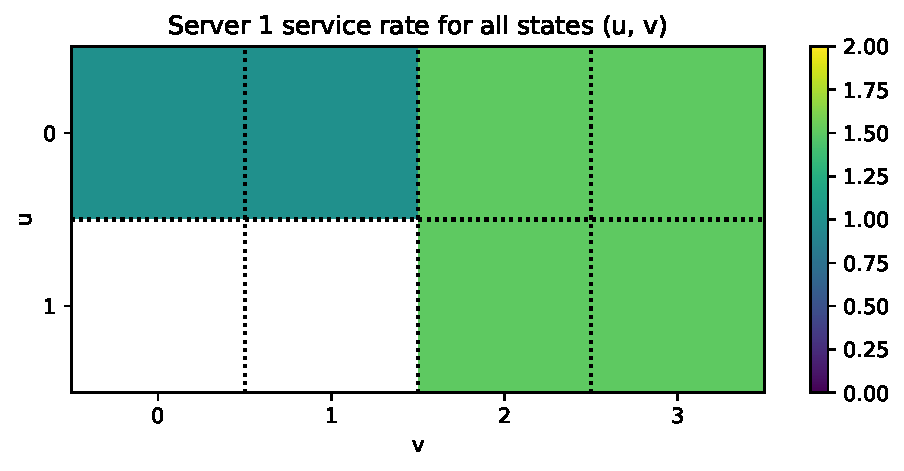
\includegraphics[width=0.45\textwidth]{chapters/06_agent_based_extension/Bin/reinforcement_learning_policy_example/server_1_1.pdf}
    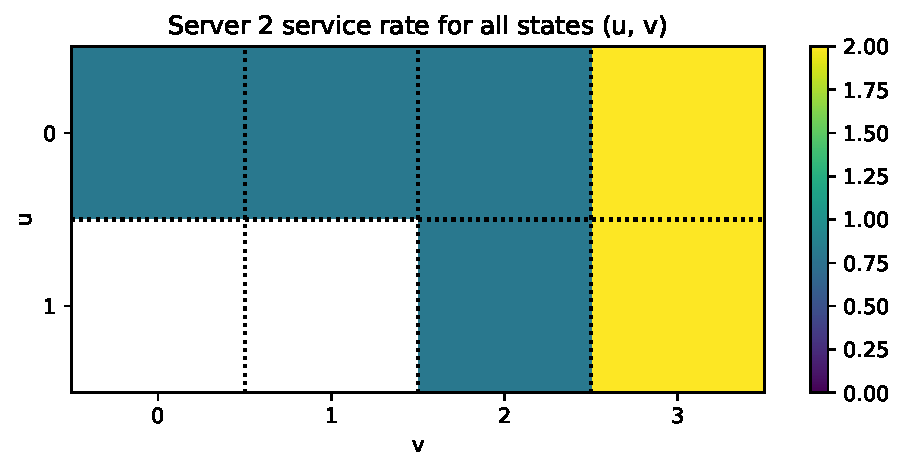
\includegraphics[width=0.45\textwidth]{chapters/06_agent_based_extension/Bin/reinforcement_learning_policy_example/server_2_1.pdf}
    \caption{Policy for server \(1\) and server \(2\) at time step \(1\)}
    \label{fig:reinforcement_learning_policy_exmaple_1}
\end{figure}


\begin{figure}[H]
    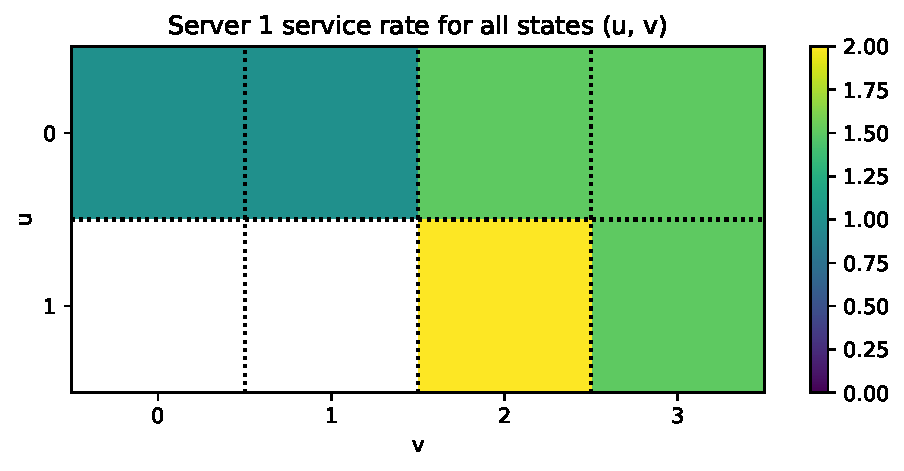
\includegraphics[width=0.45\textwidth]{chapters/06_agent_based_extension/Bin/reinforcement_learning_policy_example/server_1_2.pdf}
    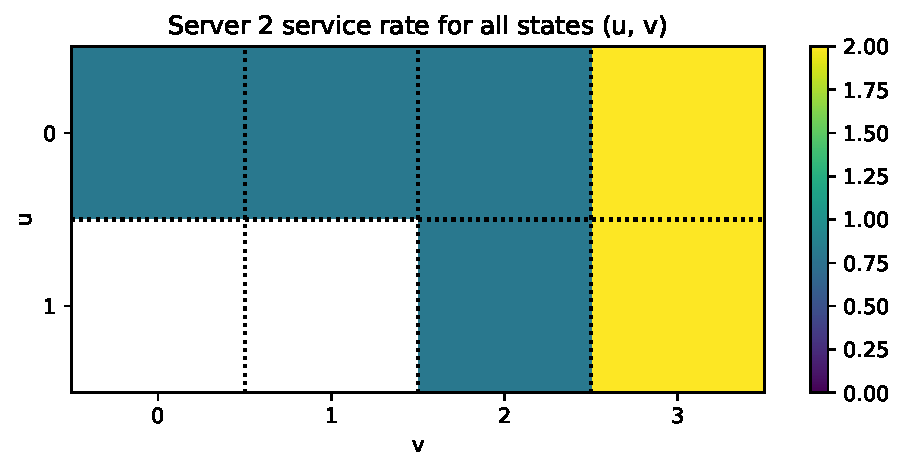
\includegraphics[width=0.45\textwidth]{chapters/06_agent_based_extension/Bin/reinforcement_learning_policy_example/server_2_2.pdf}
    \caption{Policy for server \(1\) and server \(2\) at time step \(2\)}
    \label{fig:reinforcement_learning_policy_exmaple_2}
\end{figure}

\begin{figure}[H]
    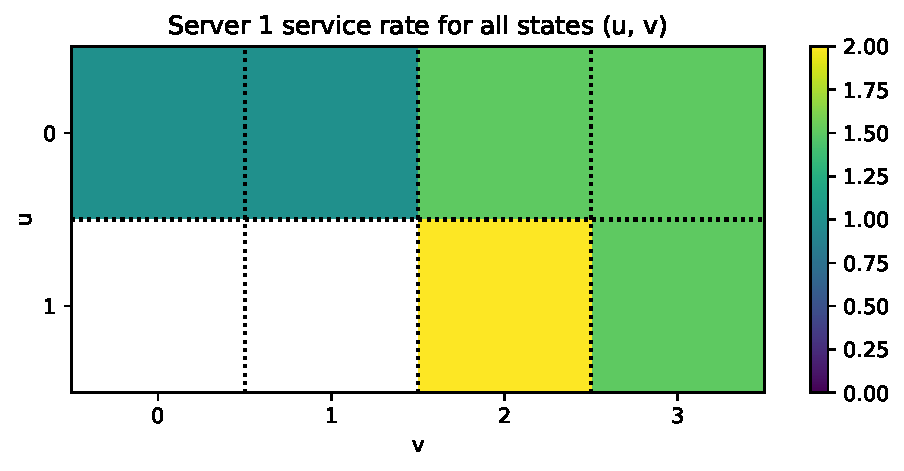
\includegraphics[width=0.45\textwidth]{chapters/06_agent_based_extension/Bin/reinforcement_learning_policy_example/server_1_3.pdf}
    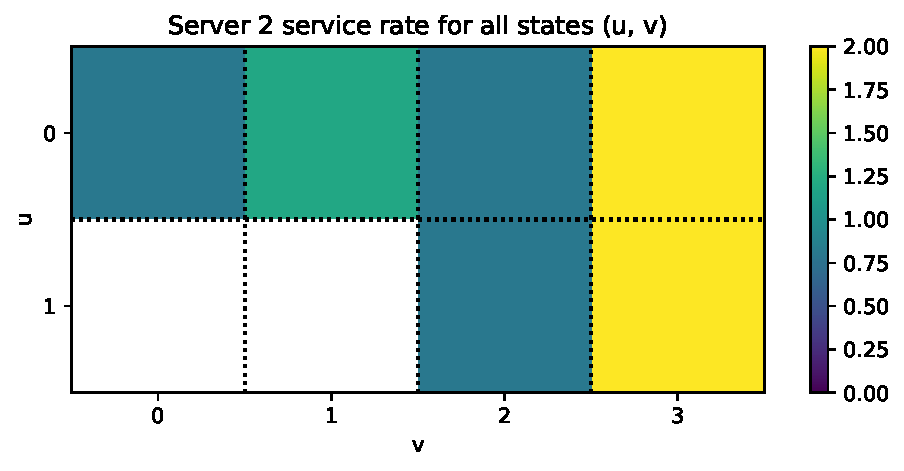
\includegraphics[width=0.45\textwidth]{chapters/06_agent_based_extension/Bin/reinforcement_learning_policy_example/server_2_3.pdf}
    \caption{Policy for server \(1\) and server \(2\) at time step \(3\)}
    \label{fig:reinforcement_learning_policy_exmaple_3}
\end{figure}



\subsection{Numeric results}\label{sec:reiforcement_learning_numeric_results}

The reinforcement learning algorithm is implemented in python and the scripts
along with the results presented in this section have been archived and can be
found in % TODO: Cite archive of scripts and results.

First and foremost, consider a queueing system with the following parameters:

\begin{multicols}{4}
    \begin{itemize}
        \item \(\lambda_2 = 1\)
        \item \(\lambda_1 = 0.5 \)
        \item \(\mu = 0.7\)
        \item \(C = 4\)
        \item \(T = 7\)
        \item \(N = 10\)
        \item \(M = 7 \)
    \end{itemize}
\end{multicols}

Note that for the initial policy, the service rates for the \(4\) servers are
set to \(0.7\) for all servers and all states.
In addition, the \(4\) servers are set to be of the same expertise level as
described in Section~\ref{sec:agent_based_case_study}.
That is, server \(1\) is an experienced server, server \(2\) and server
\(3\) are moderate servers and server \(4\) is an intern.
That means that server \(1\) is slightly faster 

% Utility function 3
%   iterations = 100000
%   e = 0, 0.1, 0.5, 1#
